\documentclass{article}
\usepackage[margin=0.80in, a4paper]{geometry} % Adjust margins here
\usepackage{amsmath}
\usepackage{float}
\usepackage{url} % For formatting URLs
\usepackage{hyperref}
\usepackage{subcaption}
\usepackage{graphicx} % subcaption for subfigure environment
\graphicspath{{./img/}}
%%%%%%%%%%%%%%%%%%%%%%%%%%%%%%%%%%%%%%%%%%%%%%%%%%%%%%%%%%%%%%%%%
\author{Francesco Angelo Fabiano Antonacci\\Francesco Sermi}

\date{\today}
\title{Relazione FFT}
%%%%%%%%%%%%%%%%%%%%%%%%%%%%%%%%%%%%%%%%%%%%%%%%%%%%%%%%%%%%%%%%%

\begin{document}
\maketitle
\section{Forme d'onda sinusoidali}

\section{Forme d'onda quadrate}

\section{Forme d'onda triangolari}

\section{Forme d'onda treni di impulsi}

\section{Forme d'onda pinne di squalo}

\section{Forme d'onda acquisite male}

\section{Forme d'onda col duty cycle}

\section{Autoscillatore}

\section{Oscillazioni smorzate}

        
        \begin{figure}[H]
            \begin{minipage}{0.45\textwidth}
                Sono state prese delle misure di segnale in uscita da un circuito RLC,
                come mostrato in Fig($\ref{fig:osc_diag}$) per tre diversi condensatori.
                Sono stati misurati il periodo e la frequenza delle oscillazioni.
                E' stato eseguito un fit ai minimi quadrati per un'oscillazione 
                smorzata per determinarne il periodo.
                E' stata eseguita una FFT per il medesimo scopo.
                I risultati sono riportati in Tab.($\ref{tab:osc_smor}$) e 
                in Fig.($\ref{fig:osc_smor}$).
            \end{minipage}%
            \hfill
            \begin{minipage}{0.45\textwidth}
                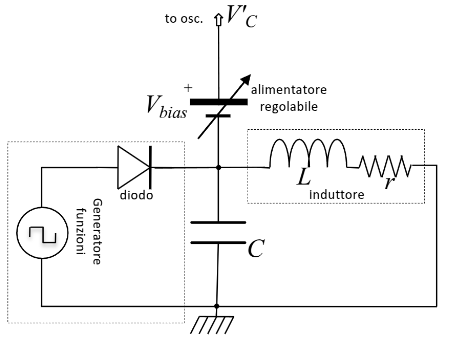
\includegraphics[width=\textwidth]{FFT12/RLCdiagram.png}
                \caption{Diagramma del circuito RLC realizzato.}
                \label{fig:osc_diag}
            \end{minipage}
        \end{figure}

        \begin{figure}[H]
            \centering
            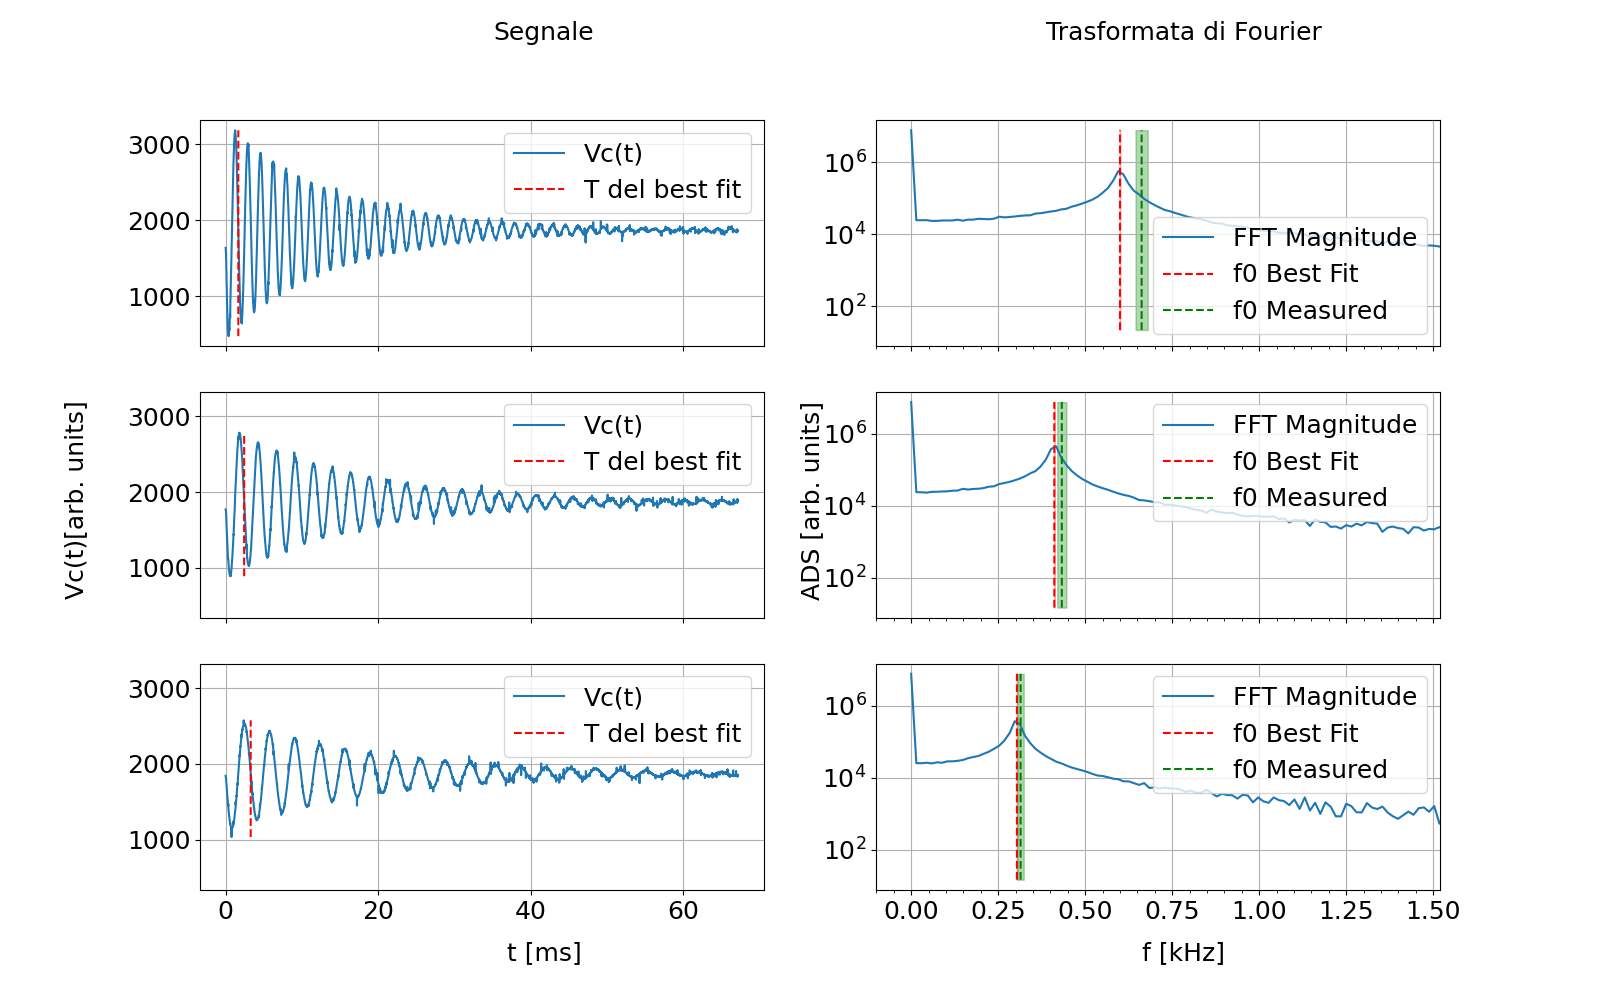
\includegraphics[width=\textwidth]{FFT12/FFTRLC.png}
            \caption{}
            \label{fig:osc_smor}
        \end{figure}

        \begin{table}[H]
            \centering
            \caption{Confronto tra le frequenze di oscillazione misurate con quelle ottenute tramite FFT e bestfit.
                    Attorno ai valori medi è stata rappresentata la barra di errore per il valore
                    misurato e per quello del bestfit, per il quale non si vede essendo molto piccola.}
                \begin{tabular}{cccc}
                    $C$[$\mu$F]          &$f_{0mis}$                &   $f_{0fft}$[kHz]       & $f_{0bestfit}$[kHz] \\
                    \hline
                    $0.1 \pm 20\%tol.$   &     $0.66 \pm 0.02$      & $0.595 \pm 0.004$       & $0.6001 \pm 0.0003$ \\
                    $0.22 \pm 20\%tol.$  &$0.43 \pm 0.01$           & $0.416 \pm 0.004$       & $0.41131\pm 0.00002$ \\
                    $0.47 \pm 20\%tol.$  &$0.314 \pm 0.009 $        &$0.298 \pm 0.004$        & $0.30393\pm 0.00002$ \\
                \end{tabular}
                \label{tab:osc_smor}

        \end{table}
    
    Le frequenze ottenute tramite la FFT e tramite il bestfit sono compatibili, 
    eccetto per la prima frequenza misurata, entro la barra di errore.

    Coerentemente con quanto ci si può aspettare sono presenti 2 picchi nella FFT,
    uno a frequenza nulla, in quanto il segnale non è alternato, l'altro
    alla frequenza di oscillazione del segnale.

    Siccome il segnale non è perfettamente sinusoidale , la FFT
    presenta un ampio spettro di armoniche attorno al picco principale.

\section{Materiali nel core dell'induttore}
    \subsection{Niente}
    \subsection{Lamine di ferro}
    \subsection{Bacchetta di ferro}
    \subsection{Parallelepipedo di alluminio}
    \subsection{Trafilato di alluminio}
    \subsection{Trafilato di alluminio segato}

\section{Glicemia}

\section{Il pinnacolo}

\end{document}